% Source: graduate-coursework/Sp26/CSCE775/course_notes/mc_prediction_guide.tex
% Description: Every-visit MC estimates. Both returns are averaged for $S_1$ and $S_2$.

\documentclass[border=4pt]{standalone}
\usepackage{amsfonts}
\usepackage{amsmath}
\usepackage{amssymb}
\usepackage{amsthm}
\usepackage[T1]{fontenc}
\usepackage{graphicx}
\usepackage{tikz}
\usepackage{xcolor}
\usetikzlibrary{arrows.meta, positioning, shapes.geometric, calc, decorations.pathreplacing}

\definecolor{Garnet}{HTML}{73000a}
\definecolor{SecondaryBlue}{HTML}{466A9F}
\definecolor{SecondaryGreen}{HTML}{65780B}
\definecolor{FlatRed}{HTML}{CC2E40}
\definecolor{FlatDark}{HTML}{1F414D}
\definecolor{FlatYellow}{HTML}{CED318}
\definecolor{FlatGold}{HTML}{A49137}
\definecolor{LightGray}{HTML}{F0F0F0}
\definecolor{Rose}{HTML}{CC2E40}

\renewcommand{\baselinestretch}{1.2}
\newcommand{\vocab}[1]{\textbf{\textcolor{Garnet}{#1}}}
\newcommand{\mathhighlight}[1]{\textcolor{SecondaryBlue}{#1}}

\begin{document}
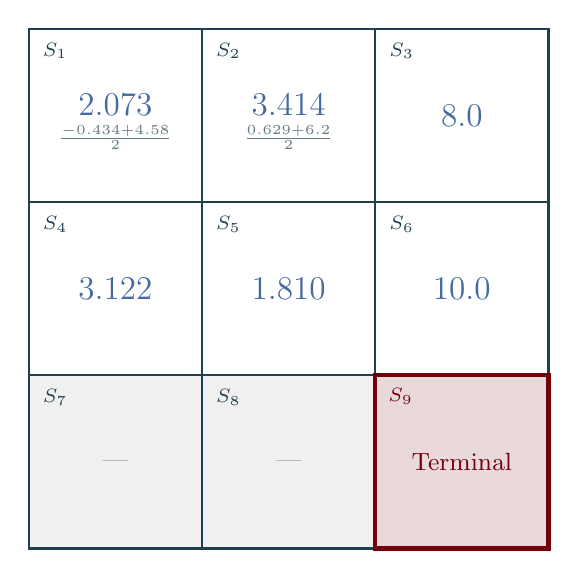
\begin{tikzpicture}[
    cell/.style={minimum size=2.2cm, draw=FlatDark, thick},
    goal/.style={cell, fill=Garnet!15, draw=Garnet, line width=1.5pt},
    empty/.style={cell, fill=LightGray},
    val/.style={font=\large\bfseries, SecondaryBlue},
    detail/.style={font=\scriptsize, FlatDark!70},
    slabel/.style={font=\scriptsize, FlatDark}
]
% Row 1
\node[cell] (s1) at (0, 4.4) {};
\node[slabel, anchor=north west] at ([shift={(2pt,-2pt)}]s1.north west) {$S_1$};
\node[val] at ([yshift=4pt]s1.center) {$2.073$};
\node[detail] at ([yshift=-8pt]s1.center) {$\frac{-0.434 + 4.58}{2}$};

\node[cell] (s2) at (2.2, 4.4) {};
\node[slabel, anchor=north west] at ([shift={(2pt,-2pt)}]s2.north west) {$S_2$};
\node[val] at ([yshift=4pt]s2.center) {$3.414$};
\node[detail] at ([yshift=-8pt]s2.center) {$\frac{0.629 + 6.2}{2}$};

\node[cell] (s3) at (4.4, 4.4) {};
\node[slabel, anchor=north west] at ([shift={(2pt,-2pt)}]s3.north west) {$S_3$};
\node[val] at (s3.center) {$8.0$};

% Row 2
\node[cell] (s4) at (0, 2.2) {};
\node[slabel, anchor=north west] at ([shift={(2pt,-2pt)}]s4.north west) {$S_4$};
\node[val] at (s4.center) {$3.122$};

\node[cell] (s5) at (2.2, 2.2) {};
\node[slabel, anchor=north west] at ([shift={(2pt,-2pt)}]s5.north west) {$S_5$};
\node[val] at (s5.center) {$1.810$};

\node[cell] (s6) at (4.4, 2.2) {};
\node[slabel, anchor=north west] at ([shift={(2pt,-2pt)}]s6.north west) {$S_6$};
\node[val] at (s6.center) {$10.0$};

% Row 3
\node[empty] (s7) at (0, 0) {};
\node[slabel, anchor=north west] at ([shift={(2pt,-2pt)}]s7.north west) {$S_7$};
\node[font=\small, FlatDark!50] at (s7.center) {---};

\node[empty] (s8) at (2.2, 0) {};
\node[slabel, anchor=north west] at ([shift={(2pt,-2pt)}]s8.north west) {$S_8$};
\node[font=\small, FlatDark!50] at (s8.center) {---};

\node[goal] (s9) at (4.4, 0) {};
\node[slabel, anchor=north west] at ([shift={(2pt,-2pt)}]s9.north west) {\textcolor{Garnet}{$S_9$}};
\node[font=\small, Garnet] at (s9.center) {Terminal};
\end{tikzpicture}
\end{document}
